\section{Shallow Neural Network}

Standalone regressions approximate data with a single function. Hence they can't represent complex patterns. 

\begin{figure}
  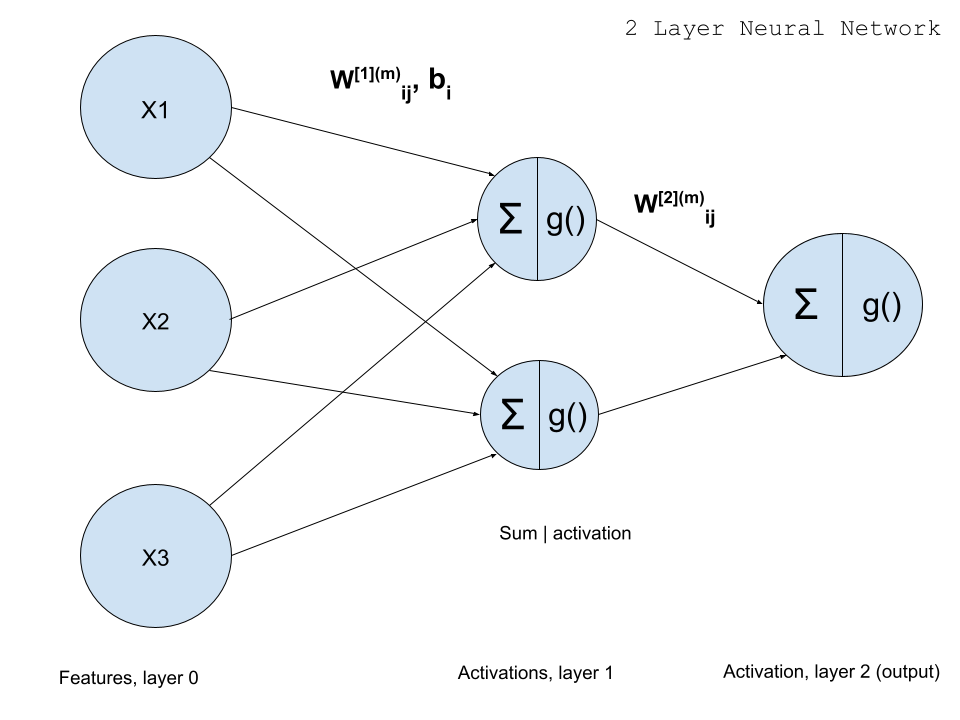
\includegraphics[width=\textwidth]{2L-NN.png}
  \caption{Shallow NN diagram}\label{fig:shallow}
\end{figure}
We calculate what is shown in \ref{fig:shallow}.

\subsection{Forward Propagation}
What changes is $W$, passes from a vector to a matrix. Each row will represent a node.

\begin{align}
  \mathbf{A} = \mathbf{W} \cdot{} \mathbf{X} + \mathbf{B} \label{eq:multi}
\end{align}

\begin{equation*}
  \begin{bmatrix}
    a_1^1 &\ldots & a_m^1\\
    a_1^2 &\ldots & a_m^2\\
    \vdots &\ldots & \vdots\\
    a_1^s &\ldots & a_m^s\\
  \end{bmatrix}
  = 
  \begin{bmatrix}
    w_1^1& w_2^1& \ldots& w_n^1\\
    w_1^2& w_2^2& \ldots& w_n^2\\
    \vdots& \vdots& \ddots& \vdots\\
    w_1^s& w_2^s& \ldots& w_n^1\\
  \end{bmatrix}
  \begin{bmatrix}
    x_{11} & x_{12} & \ldots & x_{1m}\\
    x_{21} & x_{22} & \ldots & x_{2m}\\
    \vdots & \vdots & \ddots & \vdots\\
    x_{n1} & x_{22} & \ldots & x_{nm}\\
  \end{bmatrix}
  + \begin{bmatrix}b_1\\ b_2\\ \vdots\\ b_n\end{bmatrix}
\end{equation*}

$A$ acts now like $X$, each column being a sample. Each row belongs to a node. And each activation in the row, is a linear combination of weights and bias from that node, and a sample from $X$.

This process can be done iteratively, with many layers.
\begin{itemize}
  \item Each \textit{row in the is associated with a single node} in the neural network. 
  \item Each \textit{column is instead refered to a sample} of $X$ going through each node, so it's a \textit{different linear combination of the features}. 
\end{itemize}

To look at detailed take a hidden layer with two nodes, and two initial input features.

\begin{equation*}
  \begin{bmatrix}
    a_1^1 & a_2^1\\
    a_1^2 & a_2^2\\
  \end{bmatrix}
  = 
  \begin{bmatrix}
    w_1^1& w_2^1\\
    w_1^2& w_2^2
  \end{bmatrix}
  \begin{bmatrix}
    x_{11} & x_{12}\\
    x_{21} & x_{22} 
  \end{bmatrix}
  + \begin{bmatrix}b_1\\ b_2\end{bmatrix}
\end{equation*}

They compute:

\begin{align*}
  a_1^1 &= w_1^1\,x_{11} + w_2^1\,x_{21} + b_1\\
  a^2_1 &= w_1^2\,x_{11} + w_2^2\,x_{21} + b_2\\
  a_2^1 &= w_1^1\,x_{12} + w_2^1\,x_{22} + b_1 \\
  a_2^2 &= w_1^2\,x_{12} + w_2^2\,x_{22} + b_2
\end{align*}
The upper number is the neuron, lower number is the sample. If each of those is input to a linear function the result is $r_1 = c_1\,a_1^1 + c_2\, a_1^2 + b$ and $r_2 = c_1\,a_2^1 + c_2\, a_2^2+b$ this is the same than using a single neuron. The same thing happens if we have any other linear piece like a sigmoid. Hence \textit{linear functions aren't normally used in hidden layers.}

But the whole reasoning is useful for other hidden layers.

Luckily, each activation is input to a function, hence the whole matrix is passed through a function (easy to do in python).

\subsection{Implement Forward Propagation}
In the code, we implement equation \ref{eq:multi} several times. The most important piece is:

\begin{verbatim}
# arch is an array describing the architecture:
arch = [4,3,2,1] has 4 layers with those nodes.
def fp(X, arch):
    W,B = initialize(arch[0], X.shape[0]) #nodes x features
    A = predict(W,B,X,np.tanh) # 2, m
    for layer in arch[1:-1]:
        W,B = initialize(arch[layer], A.shape[0]) 
        A = predict(W,B,A,np.tanh) # 2, m
    W,B = initialize(arch[-1], A.shape[0]) #nodes x features
    return predict(W,B,A,sigmoid)
\end{verbatim}

Sanity check: $W$, $b$ aren't initialized as zeros, but if they were and the output is a sigmoid, the result has to be $0.69$.

